\documentclass[a4paper,10pt]{article}
%DIF LATEXDIFF DIFFERENCE FILE
%DIF DEL Lspec_old.tex   Sat Mar 12 21:48:32 2016
%DIF ADD Lspec.tex       Sat Mar 12 22:02:21 2016
\usepackage[utf8]{inputenc}
\usepackage{amsthm}
\usepackage{amsmath}
\usepackage{xcolor}
\newtheorem{definition}{Definition}
\newtheorem{claim}{Claim}
\newtheorem{theorem}{Theorem}
\newtheorem{example}{Example}
\newtheorem{condition}{Condition}
\newtheorem{proposition}{Proposition}
\usepackage{graphicx}
\definecolor{mygreen}{RGB}{0,150,0}
\newtheorem{lemma}{Lemma}
\usepackage{color}
\usepackage{calrsfs}

\usepackage{latexsym}
\usepackage{listings}
\usepackage{mathrsfs}
\usepackage[colorlinks=true]{hyperref}
\hypersetup{
    colorlinks,
    citecolor=black,
    filecolor=black,
    linkcolor=blue,
    urlcolor=blue
}
\usepackage{ulem}
\def\st{\noindent}
\renewcommand\em{\it}
\renewcommand\emph{\textit}
\newcommand\red[1]{{\color{red}#1}}
\newcommand\blue[1]{{\color{blue}#1}}
\newcommand\green[1]{{\color{mygreen}#1}}
\newcommand\cancelr[1]{{\color{red}\sout{#1}}}
\newcommand\cancelg[1]{{\color{mygreen}\sout{#1}}}
%\newcommmand{\red}[1]{\textcolor{red}{#1}}
%\renewcommand\red[1]{{\color{red}#1}}
%opening
\title{L specification (draft)}
\author{Evgenii Balai}
\def\no{{ not}\;}
%DIF PREAMBLE EXTENSION ADDED BY LATEXDIFF
%DIF UNDERLINE PREAMBLE %DIF PREAMBLE
\RequirePackage[normalem]{ulem} %DIF PREAMBLE
\RequirePackage{color}\definecolor{RED}{rgb}{1,0,0}\definecolor{BLUE}{rgb}{0,0,1} %DIF PREAMBLE
\providecommand{\DIFaddtex}[1]{{\protect\color{blue}\uwave{#1}}} %DIF PREAMBLE
\providecommand{\DIFdeltex}[1]{{\protect\color{red}\sout{#1}}}                      %DIF PREAMBLE
%DIF SAFE PREAMBLE %DIF PREAMBLE
\providecommand{\DIFaddbegin}{} %DIF PREAMBLE
\providecommand{\DIFaddend}{} %DIF PREAMBLE
\providecommand{\DIFdelbegin}{} %DIF PREAMBLE
\providecommand{\DIFdelend}{} %DIF PREAMBLE
%DIF FLOATSAFE PREAMBLE %DIF PREAMBLE
\providecommand{\DIFaddFL}[1]{\DIFadd{#1}} %DIF PREAMBLE
\providecommand{\DIFdelFL}[1]{\DIFdel{#1}} %DIF PREAMBLE
\providecommand{\DIFaddbeginFL}{} %DIF PREAMBLE
\providecommand{\DIFaddendFL}{} %DIF PREAMBLE
\providecommand{\DIFdelbeginFL}{} %DIF PREAMBLE
\providecommand{\DIFdelendFL}{} %DIF PREAMBLE
%DIF END PREAMBLE EXTENSION ADDED BY LATEXDIFF
%DIF PREAMBLE EXTENSION ADDED BY LATEXDIFF
%DIF HYPERREF PREAMBLE %DIF PREAMBLE
\providecommand{\DIFadd}[1]{\texorpdfstring{\DIFaddtex{#1}}{#1}} %DIF PREAMBLE
\providecommand{\DIFdel}[1]{\texorpdfstring{\DIFdeltex{#1}}{}} %DIF PREAMBLE
%DIF END PREAMBLE EXTENSION ADDED BY LATEXDIFF

\begin{document}

\maketitle
\st
\setcounter{tocdepth}{2}
\tableofcontents
\section{Syntax}
\subsection{Symbols}\label{symbols}
L symbols are non-empty strings of ascii characters divided into the following disjoint categories:
\begin{itemize}
\item integer numerals
\item identifiers
\item special characters
\end{itemize}

\DIFaddbegin \DIFadd{An }\DIFaddend \textbf{\DIFdelbegin \textit{\DIFdel{An integer numeral}}%DIFAUXCMD
\DIFdelend \DIFaddbegin \textit{\DIFadd{integer numeral}}\DIFaddend } is a string of one or more decimal digits (0-9)\DIFdelbegin \DIFdel{possibly preceding by a minus sign
}\DIFdelend \DIFaddbegin \DIFadd{.
}\DIFaddend 


An \textbf{\textit{identifier}} is a string of one \DIFaddbegin \DIFadd{letter followed by zero }\DIFaddend or more letters, digits\DIFdelbegin \DIFdel{and underscore characters beginning with a letter}\DIFdelend \DIFaddbegin \DIFadd{, and underscores}\DIFaddend .

A \textbf{\textit{special character}} is one of the following characters:
\DIFdelbegin %DIFDELCMD < \begin{verbatim}%DIFDELCMD < 
%DIFDELCMD < '>','=','<','+','-','*','-','{','}','(',')',',','.','|'
%DIFDELCMD < \end{verbatim}
%DIFDELCMD < %%%
\DIFdelend \DIFaddbegin \begin{verbatim}
> = < + - * / % { } ( ) , . | \
\end{verbatim}
\DIFaddend 

A \textbf{\textit{symbol}} is an integer numeral, an identifier or a special character.
\subsection{Basic Terms}
Basic terms are divided into the following categories:
\begin{itemize}
\item constants
\item variables
\item typed variables
\item arithmetic terms
\item functional terms
\end{itemize}

A \textit{\textbf{constant}} is either an \DIFaddbegin \DIFadd{integer numeral or an }\DIFaddend identifier starting with a lowercase letter\DIFdelbegin \DIFdel{or an integer numeral}\DIFdelend .



A \textit{\textbf{variable}} is an identifier starting with an uppercase letter. 

A \textit{\textbf{typed variable}} is a string of the form $id~var$, where $id$ is an identifier also referred to as $type~name$ and $var$ is a variable.

An \textit{\textbf{arithmetic term}} is a string of \DIFdelbegin \DIFdel{one of the following forms: 
}%DIFDELCMD < \begin{itemize}
%DIFDELCMD < \item  %%%
\DIFdel{$-(t)$ 
}%DIFDELCMD < \item %%%
\DIFdel{$(t \diamond u)$
}%DIFDELCMD < \end{itemize} 
%DIFDELCMD < %%%
\DIFdel{where}\DIFdelend \DIFaddbegin \DIFadd{the form $t \diamond u$, where: }\DIFaddend each of $t$ and $u$ is either an integer numeral, a variable, \DIFdelbegin \DIFdel{a numeric constant  }\DIFdelend or an  arithmetic \DIFdelbegin \DIFdel{terms}\DIFdelend \DIFaddbegin \DIFadd{term}\DIFaddend ; and $\diamond$ is a special symbol in the set \texttt{\{'+', '-', '*', '/', '\%'\}} \DIFdelbegin \DIFdel{; (}\DIFdelend \DIFaddbegin \DIFadd{(with }\DIFaddend \texttt{'\%'} \DIFdelbegin \DIFdel{stands for modulo operation}\DIFdelend \DIFaddbegin \DIFadd{standing for modulo operator}\DIFaddend ). Parentheses can optionally be omitted in which case standard operator precedences apply. 

A \textbf{\textit{functional term}} is a string of the form $f(t_1,\ldots t_n)$ where $t_1,\dots,t_n$ are basic terms, f  is an identifier also referred to as \DIFdelbegin \DIFdel{an }\DIFdelend \DIFaddbegin \DIFadd{a }\DIFaddend \textit{\textbf{functional symbol}}\DIFaddbegin \DIFadd{, }\DIFaddend and $n>0$. 

\DIFaddbegin \DIFadd{Let $t$ and $t^\prime$ be basic terms. }\DIFaddend We will say that \DIFdelbegin \DIFdel{a basic term }\DIFdelend $t^\prime$ is a \textbf{\textit{subterm}} of $t$ iff at least one of the following \DIFdelbegin \DIFdel{condition }\DIFdelend \DIFaddbegin \DIFadd{conditions }\DIFaddend holds:
\begin{itemize}
\item $t  = t^\prime$ 
\item $t$ is of the form \DIFdelbegin \DIFdel{$-(t^\prime)$
}%DIFDELCMD < \item %%%
\DIFdel{$t$ is of the form $(t^\prime \diamond t_1)$
}\DIFdelend \DIFaddbegin \DIFadd{$t^\prime \diamond t_1$, where $t_1$ is some basic term
}\DIFaddend \item $t$ is of the form \DIFdelbegin \DIFdel{$(t_1 \diamond t^\prime)$
}\DIFdelend \DIFaddbegin \DIFadd{$t_1 \diamond t^\prime$, where $t_1$ is some basic term
}\DIFaddend \item $t$ is of the form $f(t_1,\ldots t_n)$ and $t^\prime \in \{t_1,\ldots,t_n\}$
\item there exists a \DIFdelbegin \DIFdel{term $t^{\prime\prime}$ }\DIFdelend \DIFaddbegin \DIFadd{basic term $t_1$ }\DIFaddend such that $t^\prime$ is a subterm of  \DIFdelbegin \DIFdel{$t^{\prime\prime}$ and  $t^{\prime\prime}$ }\DIFdelend \DIFaddbegin \DIFadd{$t_1$ and  $t_1$ }\DIFaddend is a subterm of $t$
\end{itemize}

\noindent
\DIFaddbegin \DIFadd{We say that $t^\prime$ is a }\textit{\DIFadd{proper subterm}} \DIFadd{of $t$ if $t^\prime$ is a subterm of $t$ and $t^\prime \not= t$. 
}


\DIFaddend A term $t$ is called \textbf{\textit{ground}} iff \DIFaddbegin \DIFadd{at least one of the following holds:
}\DIFaddend \begin{itemize}
\item $t$ is an identifier \DIFdelbegin \DIFdel{of }\DIFdelend \DIFaddbegin \DIFadd{or }\DIFaddend an integer numeral; or 
\item all \DIFdelbegin \DIFdel{of the }\DIFdelend \DIFaddbegin \DIFadd{proper }\DIFaddend subterms of $t$  \DIFdelbegin \DIFdel{other than $t$ itself  }\DIFdelend are ground 
\end{itemize}



\subsection{Constant Declarations}\label{cd}
A \textit{\textbf{constant declaration}} is of the form 
\begin{equation}\label{cdecl}
\texttt{const} ~c = v.
\end{equation}
where  $c$ is an identifier also referred to as  
\textbf{\textit{constant name}}  and $v$ is a ground arithmetic term, an integer numeral\DIFaddbegin \DIFadd{, }\DIFaddend or an identifier. We will say that the constant $c$ is \textit{defined} by a program if \DIFdelbegin \DIFdel{it }\DIFdelend \DIFaddbegin \DIFadd{the program }\DIFaddend contains a declaration of the form (\ref{cdecl}).
\DIFaddbegin 


\DIFaddend \subsection{Set Expressions}\label{sexpr}

A \textbf{\textit{set expression}}  is of one of the following forms:
\begin{itemize}
\item $\{t_1,t_2, \ldots, t_n\}$

 where $t_1,\ldots,t_n$ are ground terms \DIFaddbegin \DIFadd{and $n>0$}\DIFaddend . 

A shorthand $\{l..r\}$ \DIFdelbegin \DIFdel{, }\DIFdelend \DIFaddbegin \DIFadd{(}\DIFaddend where each of $l$ and $r$ is either a constant name, \DIFdelbegin \DIFdel{integer numeral }\DIFdelend \DIFaddbegin \DIFadd{an integer numeral, }\DIFaddend or a ground arithmetic term\DIFaddbegin \DIFadd{) }\DIFaddend may be used to represent the  set of all integers in the \DIFdelbegin \DIFdel{range $n..m$}\DIFdelend \DIFaddbegin \DIFadd{closed interval $[l, r]$. The numeric value represented by $l$ must be strictly less than that by $r$}\DIFaddend .

%DIF >  types have not been introduced so far, so this violates linearity 
%DIF >  moreover, this constraint is not sufficient, and the correct one can be found in section 
%DIF >  which defines a program 
%DIF > \item An identifier (the name of some type).
\DIFaddbegin 

\DIFaddend \item An identifier.
\DIFdelbegin %DIFDELCMD < 

%DIFDELCMD < %%%
\DIFdelend \item $t~$\texttt{where} $~V_1~in~type_1,\ldots, V_n~in~type_n$

where $t$ is a term, $\{V_1, \ldots, V_n\}$ is \DIFdelbegin \DIFdel{a }\DIFdelend \DIFaddbegin \DIFadd{the }\DIFaddend set of all variables occurring in $t$ and $type_1, \ldots type_n$ are identifiers. 
%DIF >  same as above
%DIF > (type names).

\item $(S_1 \diamond S_2)$ , where $S_1$ and $S_2$ are set expressions and $\diamond$ is a \DIFdelbegin \DIFdel{set theoretic operation, }\DIFdelend \DIFaddbegin \DIFadd{set-theoretic operator, denoted by }\DIFaddend one of the special characters in \DIFdelbegin \DIFdel{the set $\{+,*,/\}$}\DIFdelend \DIFaddbegin \DIFadd{$\{+, *, \backslash \}$}\DIFaddend . Parentheses can be omitted in which case $*$ and \DIFdelbegin \DIFdel{$/$ }\DIFdelend \DIFaddbegin \DIFadd{$\backslash$ }\DIFaddend have higher precedence than $+$ and all operations are left-associative.
\end{itemize}

\subsection{Type Declarations}
A \textit{\textbf{type declaration}} is of the form 
\begin{equation}\label{tdecl}
\texttt{type}~t = set\_expr.
\end{equation}
where $t$ is an identifier and $set\_expr$ is a set expression defined in section \ref{sexpr}.
We will say that the type $t$ is \textit{defined} by a program if it contains a declaration of the form (\ref{tdecl}). 

\subsection{Quantified Terms}


A \textit{\textbf{quantified term}} is of \DIFdelbegin \DIFdel{one of the forms:
 }%DIFDELCMD < \begin{itemize}
%DIFDELCMD < \item %%%
\DIFdel{$ quantifier~p $
}%DIFDELCMD < \item %%%
\DIFdel{$ \mbox{\texttt{some}}~t\_Var$
}%DIFDELCMD < \end{itemize} 
%DIFDELCMD < %%%
\DIFdelend \DIFaddbegin \DIFadd{the form:
 }$$\DIFadd{ quantifier~p }$$
\DIFaddend 



Where $quantifier$ is an identifier in the set $\{\mbox{\texttt{every}, \texttt{some}}\}$, $p$ is an identifier also referred to as \DIFaddbegin \DIFadd{the }\DIFaddend $type$ \DIFdelbegin \DIFdel{,  and $t\_Var$ is a typed variable}\DIFdelend \DIFaddbegin \DIFadd{of the quantified term}\DIFaddend .

We will refer to a quantified term starting with \DIFdelbegin \DIFdel{a }\DIFdelend \DIFaddbegin \DIFadd{the }\DIFaddend quantifier $\mbox{\texttt{some}}$($\mbox{\texttt{every}}$) as an \textbf{\textit{existentially quantified}} (\textbf{\textit{universally quantified}}) \DIFaddbegin \DIFadd{term}\DIFaddend .  


\subsection{Terms}
A \textit{\textbf{term}} is either a basic term or a quantified term.
\subsection{Atoms}

Atoms are divided into two categories:
\begin{itemize}
\item predicate atoms
\item built-in atoms
\end{itemize}

A \textit{\textbf{predicate atom}} is a string of the form $p(t_1,\ldots t_n)$ where 
$p$ is an identifier also referred to as a \textbf{\textit{predicate name}} and $t_1,\ldots,t_n$ are terms \DIFaddbegin \DIFadd{with $n \geq 0$}\DIFaddend .
A predicate atom is called \textbf{\textit{basic}} if $t_1,\ldots,t_n$ are basic terms.

A \textit{\textbf{built-in atom}} is a string of the form $t_1 \preceq t_2$ where $t_1$ and $t_2$ are \DIFaddbegin \DIFadd{basic }\DIFaddend terms and $\preceq \in$ \texttt{\{'<','>', '>=','<=','=','!='\}} is a string of special characters.

An atom is called \textbf{\textit{ground}} if all the terms occurring in the atom are ground.
\DIFaddbegin 

\subsection{\DIFadd{Literals}}

\DIFadd{A }\textit{\textbf{\DIFadd{literal}}} \DIFadd{is of one of the forms:
}

\begin{itemize}
\item \DIFadd{$a$, where $a$ is an atom
}\item \DIFadd{$\texttt{not}~b$, where $b$ is a basic atom
}\end{itemize}


\DIFaddend \subsection{Sentences}\DIFaddbegin \label{sentsec}
\DIFaddend 

A \textit{\textbf{sentence}} is either \DIFdelbegin \DIFdel{an atom }\DIFdelend \DIFaddbegin \DIFadd{a literal }\DIFaddend or an expression of the \DIFdelbegin \DIFdel{form $(not~A)$, }\DIFdelend \DIFaddbegin \DIFadd{one of the forms  }\DIFaddend $(A~or~B)$, $(A~and~B)$, where $A$ and $B$ are \DIFdelbegin \DIFdel{atoms}\DIFdelend \DIFaddbegin \DIFadd{sentences}\DIFaddend . A sentence of the form $A~and~B$
can also be written as $A, B$. Parentheses can be omitted in which case \DIFdelbegin \DIFdel{$not$ has highest precedence and }\DIFdelend \DIFaddbegin \DIFadd{$and$ has higher precedence than }\DIFaddend $or$\DIFdelbegin \DIFdel{has the lowest precedence}\DIFdelend . A sentence is called a \textbf{\textit{predicate sentence}}, if all the atoms occurring in the sentence are predicate atoms.

\subsection{Maybe \DIFdelbegin \DIFdel{Literals}\DIFdelend \DIFaddbegin \DIFadd{Constructs}\DIFaddend }

A \textbf{\DIFdelbegin \textit{\DIFdel{maybe literal}}%DIFAUXCMD
\DIFdelend \DIFaddbegin \textit{\DIFadd{maybe construct}}\DIFaddend } is of the form $$\mbox{\texttt{maybe}}~p(t_1,\ldots t_n)\DIFdelbegin \DIFdel{.}\DIFdelend $$ where $p(t_1,\ldots,t_n)$ is a basic predicate atom.

\subsection{Cardinality Constraints}

A \textit{\textbf{cardinality constraint}} is of the form 
$$v_1 <= |\{p(t_1,\ldots t_n)\}| <= v_2.$$
where
\begin{enumerate}
\item each of $v_1$ and $v_2$ is a ground arithmetic term, \DIFdelbegin \DIFdel{integer numeral }\DIFdelend \DIFaddbegin \DIFadd{an integer numeral, }\DIFaddend or a constant name, 
\item $p(t_1,\ldots,t_n)$ is a basic predicate atom.
\end{enumerate}
\subsection{Rules} \label{rl}

A \textit{\textbf{rule}} can be of \DIFdelbegin \DIFdel{the }\DIFdelend two forms:
\begin{equation}\label{eq1}
  head. 
\end{equation}

\noindent
or 
\begin{equation}
head~\mbox{\texttt{if}}~sentence.
\end{equation}

\noindent
where $head$ is one of the following:
\begin{enumerate}
\item  a predicate sentence;
\item  a maybe \DIFdelbegin \DIFdel{literal}\DIFdelend \DIFaddbegin \DIFadd{construct}\DIFaddend ;
\item  a cardinality constraint.
\end{enumerate}

\DIFaddbegin \DIFadd{and $sentence$ is a sentence defined in section (\ref{sentsec}).
We will also refer to $head$ and $sentence$ as the }\textit{\textbf{\DIFadd{head}}} \DIFadd{and the }\textit{\textbf{\DIFadd{body}}} \DIFadd{of the corresponding rule respectively.
 }

\DIFaddend \subsection{Program} \label{progdef}
A \textbf{\textit{program}} is a collection of statements, each of which is either a constant declarations, a
 type declaration, or a rule.

\noindent\vspace{0.2cm}

Constant declarations of a program must satisfy the following conditions:
\begin{enumerate}
\item Each constant name must \DIFdelbegin \DIFdel{not }\DIFdelend occur in the \DIFdelbegin \DIFdel{left hand side of a constant declarationat most once}\DIFdelend \DIFaddbegin \DIFadd{left-hand side of exactly one constant declaration}\DIFaddend .
\item Each identifier which is a subterm of the \DIFdelbegin \DIFdel{right hand }\DIFdelend \DIFaddbegin \DIFadd{right-hand }\DIFaddend side of a constant declaration must occur in the \DIFdelbegin \DIFdel{left hand }\DIFdelend \DIFaddbegin \DIFadd{left-hand }\DIFaddend side of a preceding constant declaration.   

\end{enumerate}



Type declarations of a program must satisfy the following conditions:
\begin{enumerate}
\item Each type name must occur in the \DIFdelbegin \DIFdel{left hand side of a type declarationat most once}\DIFdelend \DIFaddbegin \DIFadd{left-hand side of exactly one type declaration}\DIFaddend .
\item Each identifier occurring as  a subexpression of \DIFdelbegin \DIFdel{an expression on the right hand }\DIFdelend \DIFaddbegin \DIFadd{the right-hand }\DIFaddend side of a  type declaration must be a type name defined by a preceding type declaration. 
\end{enumerate}


Rules of a program must satisfy the following conditions:

\begin{enumerate}


\item The leftmost occurrence of any variable  $V$ in a rule \DIFdelbegin \DIFdel{is }\DIFdelend \DIFaddbegin \DIFadd{must be in the head of the rule and must be }\DIFaddend preceeded by a type name (also referred to as \textit{the type} of the variable \DIFdelbegin \DIFdel{), which can also be preceed by a quantifier.
All other occurrences of $V$ are subterms of a basic term.
}\DIFdelend \DIFaddbegin \DIFadd{in this rule).
}

\DIFaddend \item For every typed variable $t~Var$\DIFaddbegin \DIFadd{, }\DIFaddend the identifier $t$ is a type defined by the program.
\item Every identifier  occurring in the rule as a subterm of an arithmetic term is a constant name defined by the program.
\DIFdelbegin %DIFDELCMD < \item %%%
\DIFdel{Every variable occurring in a rule which does not  occur in a quantified term also occurs in the head of the rule.
}%DIFDELCMD < \item %%%
\DIFdel{Every predicate atom $p(t_1,\ldots,t_n)$ occurring in $r$ does not contain two different variables $X$ and $Y$ such that $X$ occurs in a universally quantified term $every X$ in $r$ and $Y$ occurs in an existentially quantified term $some Y$ in $r$.
}\DIFdelend \end{enumerate}
\subsection{Language Grammar}


\subsubsection{Terms}


$term$ ::= $basic\_term~|~quantified\_term$ \\ 
$basic\_term$ ::= $numeric\_constant~|~variable~|~identifier~|~identifier~variable$ \\
$~~~~~~~~~~~~~~~~~~~~~|~arithmetic\_term~|~functional\_term$\\
$ground\_term$ ::= $numeric\_constant~|~identifier~|~$ \\
$~~~~~~~~~~~~~~~~~~~~~|~ground\_arithmetic\_term~|~ground\_functional\_term$\\
$arithmetic\_term$ ::= $\texttt{-(}T0\texttt{)}~|~\texttt{-} T0 ~|~\texttt{(}T0~infix_1~T1\texttt{)}~|~\texttt{(}T1~infix_2~T2\texttt{)}~|~$ \\ $~~~~~~~~~~~~~~~~~~~~~~~~~~~~|~T0~infix_1~T1~|~T1~infix_2~T2$\\
$ground\_arithmetic\_term$ ::= $\texttt{-(}T0\_g\texttt{)}~|~\texttt{-}T0\_g~|~
\texttt{(}T0\_g~infix_1~T1\_g\texttt{)}~|~\texttt{(}T1\_g~infix_2~T2\_g\texttt{)}~|~$ \\ $~~~~~~~~~~~~~~~~~~~~~~~~~~~~|~T0\_g~infix_1~T1\_g~|~T1\_g~infix_2~T2\_g$\\


\noindent
$infix_1$ ::= $ \texttt{+} ~|~ \texttt{-} $\\
$infix_2$ ::= $ \texttt{*} ~|~ \texttt{/}~|~\texttt{\%} $\\
$infix$ ::= $infix_1~|~infix_2$\\
$T0$ ::= $T1~|~T0~infix_1~T1$\\
$T1$ ::= $T2~|~T1~infix_2~T2$ \\
$T2$ ::= $(T0)~|~variable~|~numeric\_constant~|~identifier~|~identifier~variable$ \\

\noindent
$T0\_g$ ::= $T1\_g~|~T0\_g~infix_1~T1\_g$\\
$T1\_g$::= $T2\_g~|~T1\_g~infix_2~T2\_g$ \\
$T2\_g$ ::= $(T0\_g)~|~numeric\_constant~|~identifier$ \\

\noindent
$functional\_term$ ::= $identifier~\texttt{(}~terms~\texttt{)}~$\\
$ground\_functional\_term$ ::= $identifier~\texttt{(}~ground\_terms~\texttt{)}~$\\

\noindent
$quantified\_term$ ::= \DIFdelbegin \DIFdel{$quantifier~identifier~variable~|~quantifier~identifier$}\DIFdelend \DIFaddbegin \DIFadd{$quantifier~identifier$}\DIFaddend \\
$quantifier$ ::= $\texttt{every}~|~\texttt{some}$ \\
$basic\_terms$ ::= $basic\_term~|~basic\_term\texttt{,} ~basic\_terms$ \\
$ground\_terms$ ::= $ground\_term~|~ground\_term\texttt{,} ~ground\_terms$ \\
$terms$ ::= $term~|~term\texttt{,}~ terms$ \\

\subsubsection{Constant Declarations}
$const\_decl$ ::= $\texttt{const} ~identifier \texttt{=} ground\_arithmetic\_term.~|~identifier \texttt{=} identifier.~$\\
~~~~~~~~~~$~~~~~~~~~~~~~~~~~~~~|~identifier \texttt{=} numeric\_constant.$
\subsubsection{Type Declarations}

$type\_decl$ ::= $\texttt{type}~identifier~ \texttt{=} ~set\_expr.$\\
$limit$ ::= $identifier~|~numeric\_constant~|~ground\_arithmetic\_term$\\
$set$ ::= $\texttt{\{} [ground\_terms] \texttt{\}}$ \footnote{Square brackets around $basic\_terms$ mean that $basic\_terms$ are optional, that is, $\{ \}$  is a valid expression for non-terminal $set$}\\
$range$ ::= $\texttt{\{}limit..limit\texttt{\}}$\\
$set\_expr$ ::= $ST0$ \\  
$set\_constr$ ::= $basic\_term~\texttt{where}~tvars $\\
$tvars$ ::= $tvar~|~tvar\texttt{,} tvars$\\
$tvar$ ::= $variable~\texttt{in}~identifier$  \\
$ST0$ ::= $ST1~|~ST0~\texttt{+}~ST1$\\
$ST1$ ::= $ST2~|~ST1~\texttt{*}~ST2~|~ST1~\texttt{\textbackslash}~ST2$ \\
$ST2$ ::= $\texttt{(}ST0\texttt{)}~|~set~|~range~|~set\_constr~|~identifier$  \\


\subsubsection{Atoms}
$atom$::=$predicate\_atom~|~built\_in $\\
$predicate\_atom$ ::= $identifier [\texttt{(} terms \texttt{)}]$\\
$basic\_predicate\_atom$ ::= $identifier [\texttt{(} basic\_terms \texttt{)}]$\\
$built\_in$ ::= $ basic\_term~op~basic\_term$\\
$op$ ::= $\texttt{>}~|~\texttt{<}~|~\texttt{>=}~|~\texttt{<=}~|~\texttt{=}~|~\texttt{!=}$ \\
\DIFdelbegin \subsubsection{\DIFdel{Sentences}}
%DIFAUXCMD
\addtocounter{subsubsection}{-1}%DIFAUXCMD
\DIFdelend 

\DIFdelbegin \DIFdel{$sentence$ }\DIFdelend \DIFaddbegin \subsubsection{\DIFadd{Literals}}
\DIFadd{$predicate\_literal$ }\DIFaddend ::= \DIFdelbegin \DIFdel{$s3$ }\DIFdelend \DIFaddbegin \DIFadd{$predicate\_atom~|~\texttt{not}~predicate\_atom$}\DIFaddend \\
\DIFdelbegin \DIFdel{$s3$ }\DIFdelend \DIFaddbegin \DIFadd{$literal$ }\DIFaddend ::= \DIFdelbegin \DIFdel{$s2~|~s3~\texttt{or}~s2$}\DIFdelend \DIFaddbegin \DIFadd{$atom~|~\texttt{not}~predicate\_atom$
}


\subsubsection{\DIFadd{Sentences}}
\DIFadd{$sentence$ ::= $s3$ }\DIFaddend \\
$s2$ ::= \DIFdelbegin \DIFdel{$s1~|~s2~\texttt{and}~s1~|~s2~\texttt{,}~s1$
}\DIFdelend \DIFaddbegin \DIFadd{$s2~|~s3~\texttt{or}~s2$}\DIFaddend \\
$s1$ ::= \DIFdelbegin \DIFdel{$s0~|~\texttt{not}~s0$}\DIFdelend \DIFaddbegin \DIFadd{$s1~|~s2~\texttt{and}~s1~|~s2~\texttt{,}~s1$
}\DIFaddend \\
$s0$ ::= \DIFdelbegin \DIFdel{$atom~|~\texttt{(}s3\texttt{)}$ }\DIFdelend \DIFaddbegin \DIFadd{$literal~|~\texttt{(}s3\texttt{)}$ }\DIFaddend \\
$predicate\_sentence$ ::= $predicate\_s3$ \\
\DIFdelbegin \DIFdel{$predicate\_s3$ ::= $predicate\_s2~|~predicate\_s3~\texttt{or}~predicate\_s2$}%DIFDELCMD < \\
%DIFDELCMD < %%%
\DIFdelend $predicate\_s2$ ::= \DIFdelbegin \DIFdel{$predicate\_s1~|~predicate\_s2~\texttt{and}~predicate\_s1~|~predicate\_s2~\texttt{,}~pedicate\_s1$
}\DIFdelend \DIFaddbegin \DIFadd{$predicate\_s2~|~predicate\_s3~\texttt{or}~predicate\_s2$}\DIFaddend \\
$predicate\_s1$ ::= \DIFdelbegin \DIFdel{$predicate\_s0~|~\texttt{not}~predicate\_s0$}\DIFdelend \DIFaddbegin \DIFadd{$predicate\_s1~|~predicate\_s2~\texttt{and}~predicate\_s1~|~predicate\_s2~\texttt{,}~pedicate\_s1$
}\DIFaddend \\
$predicate\_s0$ ::= \DIFdelbegin \DIFdel{$predicate\_atom~|~\texttt{(}predicate\_s3\texttt{)}$ 
}\DIFdelend \DIFaddbegin \DIFadd{$predicate\_literal~|~\texttt{(}predicate\_s3\texttt{)}$ 
}\DIFaddend 


\subsubsection{Maybe \DIFdelbegin \DIFdel{Literals}\DIFdelend \DIFaddbegin \DIFadd{Statements}\DIFaddend }
\DIFdelbegin \DIFdel{$maybe\_lit$ }\DIFdelend \DIFaddbegin \DIFadd{$maybe\_st$ }\DIFaddend ::= $\texttt{maybe}~basic\_predicate\_atom$\\
\subsubsection{Cardinality Constraints}
$bound$ ::= $arithmetic\_term~|~numeric\_constant~|~identifier$\\
$card\_constr$ ::= $bound~ \texttt{<= |\{}  basic\_predicate\_atom \texttt{\}| <=} ~bound$\\

\subsubsection{Rules}
$rule$ ::= $head \texttt{.} | head~\texttt{if}~sentence \texttt{.} $ \\
$head$ ::= \DIFdelbegin \DIFdel{$predicate\_sentence~|~maybe\_lit~|~card\_constr$
 }\DIFdelend \DIFaddbegin \DIFadd{$predicate\_sentence~|~maybe\_st~|~card\_constr$
 }\DIFaddend 

\subsubsection{Program}
$program$ ::= $statements$\\
$statements$ ::= $statement~|~statement,~statements$\\
$statement$ ::= $ const\_decl~|~type\_decl~|~rule$ 


\subsection{Comments}

L programs can have comments starting with \texttt{/*} and ending with \texttt{*/} . For example:

\begin{verbatim}
/*
 This is a
 multiline comment
*/
type t = {1,2,3}. /* this is a type declaration */
p(t X) if /* this is a rule */ q(X). 
\end{verbatim}


\section{Semantics}
We define the semantics of an $L$ program $\Pi$ in terms of \textit{models} of $P$. A model is\DIFdelbegin \DIFdel{a }\DIFdelend \DIFaddbegin \DIFadd{, intuitively,  a minimal }\DIFaddend set of atoms which, \DIFdelbegin \DIFdel{intuitively, }\DIFdelend satisfies the rules of the program. 
The notion of satisfiability is defined in section \ref{rsat} with all necessary background provided in sections 
\ref{constants} - \ref{grp}.

The semantics of a program $P$ containing \DIFdelbegin \DIFdel{a comment }\DIFdelend \DIFaddbegin \DIFadd{comments }\DIFaddend coincide with the semantics of the program obtained from $P$ by removing the comments. In the rest of this section we will consider programs not containing comments.




\subsection{Constant Declarations} \label{constants}


Let $\Pi$ be an $L$ program starting with \DIFaddbegin \DIFadd{a }\DIFaddend constant declaration of the form
$$\texttt{const} ~cn = gar\_term.$$

Where $cn$ is referred to as a constant name and $gar\_term$ is a ground arithmetic term.
By condition 2 for constant declarations defined in section \ref{progdef}, $gar\_term$ cannot contain identifiers as subterms,
therefore its value $v$ can be obtained as defined in section \ref{at}. 

The models $\Pi$ coincide with the models of program $\Pi^\prime$ obtained from $\Pi$ by:
\begin{enumerate}
\item Removing the declaration $\texttt{const}~cn = gar\_term.$
\item Replacing every subterm of a term \DIFaddbegin \DIFadd{in }\DIFaddend $\Pi$ equal to $cn$ with \DIFaddbegin \DIFadd{the }\DIFaddend numeric constant $v$. 
\end{enumerate} 


\medskip\noindent
By condition 2 for constant declarations defined in section \ref{progdef}, if the program $\Pi^\prime$ starts another constant declaration, its right hand side cannot contain numeric constants, therefore its semantics can be defined in the same manner as for $\Pi$.

\medskip\noindent
Therefore, it is sufficient to define the semantics for programs not containing constant declarations (and, therefore, not containing constant names in arithmetic terms \DIFdelbegin \DIFdel{too}\DIFdelend \DIFaddbegin \DIFadd{either}\DIFaddend ).

\subsection{Arithmetic Terms}\label{at}

A program may contain ground arithmetic terms constructed from integer numerals and operations `+` (plus),  `-` (minus), `*` (multiplication), `/` (integer division), `\%` (modulo)\footnote{Current implementation allows only numerals in the range \DIFdelbegin \DIFdel{-2,147,483,648 }\DIFdelend \DIFaddbegin \DIFadd{from 0 }\DIFaddend to 2,147,483,647. Moreover, correct evaluation for an arithmetic term is guaranteed only if all its subterms have values within the range.} Each arithmetic term  has \textit{a value}. 
The meaning and precedence of operations  `+`,  `-`, `*` is as usual. The  operation `/` has the same precedence as `*` and is defined as $$a/b := sgn(a*b) *(|a|~div~|b|)$$
where 
\begin{enumerate}
\item $sgn(a*b) = \begin{cases} 1 &\mbox{if } a *b \ge 0 \\
-1 & \mbox{otherwise }. \end{cases} $
\item for $a\ge 0$ and $b\ge0$ $a~div~b$ is a floor division, i.e, $a~div~b$ is the largest integer such that $b * (a~div~b)  \le  a$.
\end{enumerate}
The  operation `/` has the same precedence as `*` and is defined as $$a\%b := a - n * (a/n) $$
All operations are associated from left to right. 


\medskip\noindent
The semantics of programs containing undefined arithmetic operations (division by zero or modulo with its second operand equal to zero) is undefined.  

  


\subsection{Type Declarations} \label{types}
Type declarations of a program $\Pi$  define a mapping $\mathcal{D}_\Pi$ from identifiers (also called type names) and set expressions of $\Pi$  to sets of ground terms. If $q$ is a type name or a sort expression, $\mathcal{D}_\Pi(q)$  denotes the set of ground terms it is mapped to. 


\medskip\noindent 
The mapping is defined as follows:

\begin{enumerate}
\item For every sort expression of the form $$\{t_1,\ldots,t_n\}$$   $\mathcal{D}_\Pi(\{t_1,\ldots,t_n\})$ is $ \{t_1,\ldots,t_n\}$
\item For every sort expression of the form   $$t~\mbox{\texttt{where}} ~V_1~in~type_1,\ldots, V_n~in~type_n$$

\noindent
$\mathcal{D}_\Pi(t~\mbox{\texttt{where}} ~V_1~in~type_1,\ldots, V_n~in~type_n)$ is $\{t| V_1 \in \mathcal{D}_\Pi(type_1),\ldots, V_n \in \mathcal{D}_\Pi(type_n)\}$ 
\item For every \DIFdelbegin \DIFdel{sort }\DIFdelend \DIFaddbegin \DIFadd{set }\DIFaddend expression of the form $$S_1 \diamond S_2$$ 
$\mathcal{D}_\Pi(S_1 \diamond S_2)$ is $ \mathcal{D}_\Pi(S_1) \odot  \mathcal{D}_\Pi(S_2)$, where $\odot$ is a set operation: union, intersection, or difference when $\diamond$ is $+$, $*$ or \DIFdelbegin \DIFdel{$/$ }\DIFdelend \DIFaddbegin \DIFadd{$\backslash$ }\DIFaddend correspondingly.

\item For every type declaration of the form $$\texttt{type}~tn = set\_expr$$

$\mathcal{D}_\Pi(tn)$ is $\mathcal{D}_\Pi(set\_expr)$  


\end{enumerate}

\medskip\noindent
In the remainder of the section  we will mostly  use   $\mathcal{D}_\Pi$ to obtain the values  which correspond to the type names of $\Pi$.


%DIF > VUUUUUUUUUUUUUU
\subsection{Programs with \DIFdelbegin \DIFdel{Free }\DIFdelend Variables and Ground Programs}\label{grp}

\DIFdelbegin \DIFdel{Let $\Pi$ be an $L$ program and $r$ be a rule of $P$. 
A variable $V$ occurring in  $r$  is called a }\textit{\DIFdel{free}} %DIFAUXCMD
\DIFdel{variable if at least one of the following conditions is satisfied:
}%DIFDELCMD < \begin{enumerate}
%DIFDELCMD < \item %%%
\DIFdel{$V$ occurs in the  head of $r$, and the head of $r$ is either a sentence or a maybe literal.
}%DIFDELCMD < \item %%%
\DIFdel{$V$ occurs in the head of $r$ and in the body of $r$.
}%DIFDELCMD < \end{enumerate}
%DIFDELCMD < %%%
\DIFdel{Other variables occurring in $r$ are }\textit{\DIFdel{quantified}} %DIFAUXCMD
\DIFdel{variables.
}%DIFDELCMD < 

%DIFDELCMD < %%%
\DIFdelend For a program $\Pi$ \DIFaddbegin \DIFadd{containing variables }\DIFaddend we obtain a corresponding \textit{ground} program $\Pi^g$ as follows:
\begin{enumerate}
\item each rule $r$ containing \DIFdelbegin \DIFdel{free }\DIFdelend variables is replaced with a maximal collection of rules, each of which corresponds to a unique substitution 
of  \DIFdelbegin \DIFdel{free }\DIFdelend variables (together with possibly preceeding type names)  with ground terms. A variable $v$ can be replaced with a term $f$ if
\begin{itemize}
\item there in an occurrence of a typed variable $t~v$ in $r$, and
\item  $f\in \mathcal{D}(t)$
\end{itemize}  
\item each arithmetic term is evaluated as described in section  \ref{at}.
\end{enumerate}

\medskip\noindent
For example, consider the program 
\begin{verbatim}
type type1 = {1,2,5}.
type type2 = {1,2}.

p(type1 X, type2 Y) if X+Y = 7.
maybe q(type1 X).
1<=|{t(type1 X, type2 Y)}| <= 2 if q(Y).
\end{verbatim}

\medskip\noindent
The corresponding ground program is:
\begin{verbatim}
p(1, 1) if 2 = 7
p(1, 2) if 3 = 7
p(2, 1) if 3 = 7
p(2, 2) if 4 = 7
p(5, 1) if 6 = 7
p(5, 2) if 7 = 7
maybe q(1).
maybe q(2).
maybe q(5).
1<=|{t(type1 X, 1)}| <= 2 if q(1).
1<=|{t(type1 X, 2)}| <= 2 if q(2).
\end{verbatim}

\medskip\noindent
Therefore, any program $\Pi$ can be viewed as a shorthand for the corresponding ground program $\Pi^g$.
In the following sections we will define the semantics of ground programs.


\subsection{Program Models}\label{rsat}
A model of $\Pi$ is a set of ground atoms satisfying certain conditions.

To describe the conditions,  we  first introduce some definitions.
 We will call a predicate atom $p(t_1,\ldots, t_n)$ \textit{basic} if all the terms $t_1,\ldots t_n$ are basic.
 \DIFaddbegin 

\DIFaddend Similarly, a sentence is called basic if all the atoms occurring in the sentence are basic.

\begin{definition}(A set ground atoms satisfying a basic predicate atom) \\
\rm{
A set of ground atoms $A$ satisfies a simple predicate atom $p(t_1,\ldots t_n)$  if and only if $p(t_1,\ldots t_n) \in A$.
%Let $A$ be a set of ground atoms and $p(t_1,\ldots,t_n)$ be a predicate atom.
%Let $E = [e_1,\ldots,e_k]$ be a set of all natural numbers in $[1..n]$ such that for every $j \in E$ $t_j$ is an existentially %quantified term. Similarly, let  
}

\hfill$\Box$
\end{definition}

\begin{definition} (A set of ground atoms satisfying a built-in  atom)\\
{\rm
A set of ground atoms satisfies a ground built-in atom $t_1 \diamond t_2$ iff one of the following conditions is satisfied:
\begin{enumerate}
\item $\diamond$ is $=$($\not =$) and $t_1 = t_2$($t_1 \not= t_2$);
\item $\diamond$ is $<$ ($\le,\ge, >$), $t_1$ and $t_2$ are integer numerals representing numbers $N_1$ and $N_2$ respectively and
 $N_1 < N_2$ ($N_1 \le N_2, N_1 \ge N_2, N_1 > N_2$);
\item $\diamond$ is $<$ ($\le,\ge, >$),  $t_1$ and $t_2$ are identifiers starting with a lowercase letter, and $t_1$  lexicographically smaller than (smaller than or equal to, greater than or equal to, greater) $t_2$.
\end{enumerate}
} 


\hfill$\Box$
\end{definition}

\medskip\noindent
The semantics of a program containing a built-in atom $t_1 \diamond t_2$ where $\diamond~\in~\{<, \le, \ge, >\}$ is \textit{defined} if and only of both $t_1$, $t_2$ are both constants or integer numerals.

\begin{definition} (A set of ground atoms satisfying a \DIFaddbegin \DIFadd{literal)}\\
{\rm
\DIFadd{A set of ground atoms $A$ satisfies a literal $l$ if one of the following conditions is satisfied:
}\begin{enumerate}
\item \DIFadd{$l$ is of the form $a$, where $a$ is an atom satisfied by $A$
}\item \DIFadd{$l$ is of the form $\texttt{not}~a$, where $a$ is an atom not satisfied by $A$ 
}\end{enumerate}
} 
\end{definition}

\begin{definition}\DIFadd{(A set of ground atoms satisfying a }\DIFaddend basic sentence) \\
\DIFdelbegin %DIFDELCMD < \rm{
%DIFDELCMD < A set of of ground atoms $A$ satisfies a basic sentence $S$ ($A \vdash S$) if one of the following conditions is satisfied:
%DIFDELCMD < \begin{enumerate}
%DIFDELCMD < \item $S$ is a basic atom, and $S \in A$
%DIFDELCMD < \item $S$ is of the form $not~S^\prime$, and $A$ does not satisfy $S^\prime$
%DIFDELCMD < \item $S$ is of the form $S_1~or~S_2$ ($S_1~and~S_2$) and $A$ satisfies one (both) of the sentences  $S_1$ and $S_2$
%DIFDELCMD < \end{enumerate}
%DIFDELCMD < }
%DIFDELCMD < %%%
\DIFdelend \DIFaddbegin \rm{
A set of of ground atoms $A$ satisfies a basic sentence $S$ ($A \vdash S$) if one of the following conditions is satisfied:
\begin{enumerate}
\item $S$ is a literal satisfied by $A$
\item $S$ is of the form $S_1~or~S_2$ ($S_1~and~S_2$) and $A$ satisfies one (both) of the sentences  $S_1$ and $S_2$
\end{enumerate}
}
\DIFaddend 

\hfill$\Box$
\end{definition}

\noindent
\DIFdelbegin %DIFDELCMD < \medskip
%DIFDELCMD < %%%
\DIFdelend Let $S$ be a sentence. \DIFdelbegin \DIFdel{By $S^\prime$ we denote the sentence obtained from $S$ by replacing each  quantified term 
}\begin{displaymath}\DIFdel{quantifier~p }\end{displaymath}
%DIFAUXCMD
\DIFdel{with }\begin{displaymath}\DIFdel{ quantifier~p~X}\end{displaymath}
 %DIFAUXCMD
\DIFdel{where $X$ is a variable not occurring in $S$ and unique for each quantified term in $S$.
}%DIFDELCMD < 

%DIFDELCMD < \noindent\medskip
%DIFDELCMD < %%%
\DIFdel{Let
}\DIFdelend \DIFaddbegin \DIFadd{And let
}\DIFaddend \begin{itemize}
\item \DIFdelbegin \DIFdel{$X_1,\ldots X_n$ be the variables occurring in existentially }\DIFdelend \DIFaddbegin \DIFadd{$\{U_1,\ldots U_n\}$ be the set of all universally }\DIFaddend quantified terms  of \DIFdelbegin \DIFdel{$S^\prime$ of types $Tx_1,\ldots, Tx_n$ correspondingly
}\DIFdelend \DIFaddbegin \DIFadd{$S$ whose  types are $Tu_1,\ldots, Tu_n$ respectively;
}\DIFaddend \item \DIFdelbegin \DIFdel{$Y_1, \ldots Y_m$ be the variables occurring in universally }\DIFdelend \DIFaddbegin \DIFadd{$\{E_1, \ldots E_m\}$ be the set of all existentially }\DIFaddend quantified terms  of \DIFdelbegin \DIFdel{$S^\prime$ of types $Ty_1, \ldots, Ty_m$ correspondingly
}\DIFdelend \DIFaddbegin \DIFadd{$S$ whose  types are $Te_1,\ldots, Te_m$ respectively;
}\DIFaddend \end{itemize}
\DIFdelbegin %DIFDELCMD < 

%DIFDELCMD < %%%
\DIFdelend %DIF > VUUUUUUUUUUUU
\noindent\medskip
For a \DIFdelbegin \DIFdel{sentence }\DIFdelend \DIFaddbegin \DIFadd{set $\{T_1,\ldots,T_k\}$ of quantified terms of }\DIFaddend $S$\DIFdelbegin \DIFdel{by $S|_{\{Z_1 = z_1, \ldots, Z_n = z_n\}}$ }\DIFdelend \DIFaddbegin \DIFadd{,  }\DIFaddend we denote the sentence obtained from $S$ by \DIFdelbegin %DIFDELCMD < \begin{enumerate}
%DIFDELCMD < \item %%%
\DIFdel{for each variable $Z_i \in \{Z_1,\ldots, Z_n\}$ }\DIFdelend replacing every occurrence of a quantified term \DIFdelbegin \begin{displaymath}\DIFdel{ quantifier~p~Z_i}\end{displaymath} %DIFAUXCMD
\DIFdel{with $z_i$;
}%DIFDELCMD < \item %%%
\DIFdel{replacing all other occurrences of each $Z_i \in  \{Z_1,\ldots, Z_n\}$ with $z_i$.
}%DIFDELCMD < \end{enumerate}
%DIFDELCMD < %%%
\DIFdelend \DIFaddbegin \DIFadd{$T_i$  with $t_i$ by $S|_{\{T_k = t_1, \ldots, T_k = t_k\}}$.
}\DIFaddend 

\begin{definition}(A set of ground atoms satisfying a sentence)\\
\DIFdelbegin %DIFDELCMD < \rm{
%DIFDELCMD <    A set of ground terms $A$ satisfies  $S$ iff
%DIFDELCMD <   \begin{displaymath} \exists (x_1,\ldots,x_n)  \in \mathcal{D}(Tx_1) \times \ldots \times \mathcal{D}(Tx_n): 
%DIFDELCMD < \forall (y_1,\ldots,y_m) \in  \mathcal{D}(Ty_1) \times \ldots \times \mathcal{D}(Ty_m):\end{displaymath} \begin{displaymath}(A \vdash S^\prime|_{\{X_1 = x_1, \ldots, X_n = x_n, Y_1 = y_m,\ldots Y_m = y_m\}})\end{displaymath}
%DIFDELCMD < }
%DIFDELCMD < %%%
\DIFdelend \DIFaddbegin \rm{
   A set of ground terms $A$ satisfies  $S$ iff
  $$ \exists (e_1,\ldots,e_n)  \in \mathcal{D}(Te_1) \times \ldots \times \mathcal{D}(Te_n): 
\forall (u_1,\ldots,u_m) \in  \mathcal{D}(Tu_1) \times \ldots \times \mathcal{D}(Tu_m):$$ $$(A \vdash S|_{\{E_1 = e_1, \ldots, E_m = e_m, U_1 = u_1,\ldots U_n = u_n\}})$$
}
\DIFaddend 

\hfill$\Box$
\end{definition}

\begin{definition}(A set of ground atoms satisfying a cardinality constraint)\\
\rm{
Let $A$ be a set of ground atoms and $$v_1 <= |\{p(t_1,\ldots t_n)\}| <= v_2.$$ be a cardinality constraint of a program $\Pi$.
Let $X_1\ldots,X_n$ be all variables occurring in the constraint and $Tx_1,\ldots Tx_n$ be the types of the variables $X_1\ldots,X_n$ correspondingly. Let $S$ be a set of ground atoms of $\Pi$ of the form $p(t_1^\prime,\ldots t_n^\prime)$ each of which is obtained from $p(t_1,\ldots t_n)$ by replacing all occurrences of variables  with elements of their corresponding types.

\noindent\medskip
$A$ satisfies  the constraint $v_1 <= |\{p(t_1,\ldots t_n)\}| <= v_2$ iff $v_1 \le |S| \le v_2$. 

\hfill$\Box$

}
\end{definition}


As described in section \ref{rl}, program rules may be in one of the two forms. We sometimes say that a rule of the form $$head.$$ has a body which is satisfied by any set of ground atoms and use \DIFdelbegin \DIFdel{a }\DIFdelend \DIFaddbegin \DIFadd{the }\DIFaddend canonical form $$head~\mbox{\texttt{if}}~body.$$ even if the body is not present.



\begin{definition}(A set of ground atoms satisfying a rule)\\
\DIFdelbegin %DIFDELCMD < \rm{
%DIFDELCMD < A set of ground atoms $A$ satisfies a rule 
%DIFDELCMD <  head is either a cardinality constraint or a sentence and one of the following conditions holds:
%DIFDELCMD < \begin{enumerate}
%DIFDELCMD < \item $A$ does not satisfy $body$;
%DIFDELCMD < \item $A$ satisfies both $body$ and $head$.
%DIFDELCMD < \end{enumerate}
%DIFDELCMD < }
%DIFDELCMD < %%%
\DIFdelend \DIFaddbegin \rm{
A set of ground atoms $A$ satisfies a rule, whose head is either a cardinality constraint or a sentence, if one of the following conditions holds:
\begin{enumerate}
\item $A$ does not satisfy $body$;
\item $A$ satisfies both $body$ and $head$.
\end{enumerate}
}
\DIFaddend \hfill $\Box$
\end{definition}




\DIFdelbegin %DIFDELCMD < \begin{definition}%%%
\DIFdel{(A model of a program)}%DIFDELCMD < \\
%DIFDELCMD < \rm{
%DIFDELCMD < Let $A$ be a set of ground atoms of a program $\Pi$; $M$ be the sets of all literals $l$ such that $\Pi$ contains a rule
%DIFDELCMD < \begin{displaymath}\mbox{\texttt{maybe}}~l~\mbox{\texttt{if}}~body.\end{displaymath} where $body$ is satisfied by $A$.
%DIFDELCMD < $A$ is a model of $\Pi$ if and only if it can be written as a union  $M^\prime \cup C$, where
%DIFDELCMD < \begin{enumerate}
%DIFDELCMD < \item $M^\prime$ is $M \cap A$;
%DIFDELCMD < \item $C$ is the smallest set of ground literals such that $M^\prime \cup C$ satisfies all the rules of $\Pi$ whose heads are sentences;
%DIFDELCMD < \item $M^\prime \cup C$ satisfies all the rules of $\Pi$ whose heads are cardinality constraints.
%DIFDELCMD < \end{enumerate}
%DIFDELCMD < }
%DIFDELCMD < \hfill %%%
\DIFdel{$\Box$
}%DIFDELCMD < \end{definition}
%DIFDELCMD < %%%
\subsection*{\DIFdel{Alternative Definition for program models(by Dr.Gelfond)}}
%DIFAUXCMD
\DIFdelend \DIFaddbegin \subsection{\DIFadd{Program models}}
\DIFaddend 

\DIFdelbegin %DIFDELCMD < \begin{definition}%%%
\DIFdel{(Program reduct) }%DIFDELCMD < \\
%DIFDELCMD < \rm{
%DIFDELCMD < Let $\Pi$ be an L program and $A$ be a set of ground atoms.
%DIFDELCMD < We obtain an L program $\Pi^A$ (the \textit{reduct} of $\Pi$ with respect to $S$) from $\Pi$ as follows:
%DIFDELCMD < \begin{enumerate}
%DIFDELCMD < \item For every rule  $r$ of $\Pi$ of the form
%DIFDELCMD < \begin{displaymath}\mbox{\texttt{maybe}}~l~\mbox{\texttt{if}}~body.\end{displaymath} 
%DIFDELCMD < if $body$ is satisfied by $S$, add the rule $l~ \texttt{if} body$ and remove $r$.
%DIFDELCMD < \item For every rule  $r$ of $\Pi$ of the form
%DIFDELCMD < \begin{displaymath}\mbox{\texttt{maybe}}~l~\mbox{\texttt{if}}~body.\end{displaymath}  where $body$ is not satisfied by $S$, remove $r$.
%DIFDELCMD < \end{enumerate}
%DIFDELCMD < }
%DIFDELCMD < \hfill%%%
\DIFdel{$\Box$
}%DIFDELCMD < \end{definition}
%DIFDELCMD < %%%
\DIFdel{Note that the reduct of }\DIFdelend \DIFaddbegin \DIFadd{Let }\DIFaddend $\Pi$ \DIFdelbegin \DIFdel{is }\DIFdelend \DIFaddbegin \DIFadd{be }\DIFaddend an $L$ program\DIFdelbegin \DIFdel{not containing rules with maybe literals in heads.
}\DIFdelend \DIFaddbegin \DIFadd{.
For every atom $a$ occurring, let $a^\prime$ be a fresh atom not occurring in $\Pi$, such that for any two distict atoms $a_1 \not= a_2$ of $\Pi$, $a^\prime_1 \not= a^\prime_2$.
By $\Pi^\prime$ we denote a program obtained form $\Pi$ by:
}

\begin{enumerate}
\item \DIFadd{replacing all maybe contructs of the form $\texttt{maybe}~l$ with $l~or~(\texttt{not}~l)$.
}\item \DIFadd{replacing all literals of the form $\texttt{not}~a$ with $a^\prime$. 
}\end{enumerate}

\noindent
\DIFadd{Let $A^\prime$ denote the set of all new atoms introduced in $P^\prime$.
}


\DIFaddend \begin{definition}(A model of a program)\\
\DIFdelbegin %DIFDELCMD < \rm{
%DIFDELCMD < Let $A$ be a set of ground atoms of a program $\Pi$; $A$ is a model of $\Pi$ if and only if the following conditions are satisfied:
%DIFDELCMD < \begin{enumerate}
%DIFDELCMD < \item $A$ is the mimimal set satisfying the rules of $\Pi^A$ whose heads are sentences.
%DIFDELCMD < \item $A$ satisfies all the rules of $\Pi^A$ whose heads are cardinality constraints.
%DIFDELCMD < \end{enumerate}
%DIFDELCMD < }
%DIFDELCMD < %%%
\DIFdelend \DIFaddbegin \rm{
Let $A$ be a set of ground atoms of a program $\Pi$; $A$ is a model of $\Pi$ if and only if 
there exists a set of atoms $B$ of $\Pi^\prime$ such that  the following conditions are satisfied:
\begin{enumerate}
\item $A = B \setminus A^\prime$.
\item $B$ is the mimimal set satisfying the rules of $\Pi^\prime$ whose heads are predicate sentences.
\item $B$ satisfies all the rules of $\Pi^\prime$ whose heads are cardinality constraints.
\end{enumerate}
}
\DIFaddend \hfill$\Box$
\end{definition}

\section{Examples}

\subsection{Simple Examples} 

The program $\Pi_1$:
\begin{verbatim}
a.
b if a.
\end{verbatim}
has exactly one model $\{a,b\}$.

\medskip\noindent
The program $\Pi_2$:
\begin{verbatim}
a if b.
\end{verbatim}
has exactly one model $\{\}$, because it  does not contain maybe literals or cardinality constraints, and $\{\}$ is the minimal set of atoms satisfying the only rule of the program.

\medskip\noindent
The program $\Pi_3$:
\DIFdelbegin %DIFDELCMD < \begin{verbatim}%DIFDELCMD < 
%DIFDELCMD < 

%DIFDELCMD < type t1 = {5,6,7}.
%DIFDELCMD < type t2 = {0,1,2}
%DIFDELCMD < p(t2 N) if q(N+5).
%DIFDELCMD < maybe q(t1 N).
%DIFDELCMD < 1{q(t1 N)}2. 
%DIFDELCMD < \end{verbatim}
%DIFDELCMD < %%%
\DIFdel{has three models:
}%DIFDELCMD < \begin{verbatim}%DIFDELCMD < 
%DIFDELCMD < {q(5),q(6),p(1),p(0)}; 
%DIFDELCMD < {q(6),q(7),p(1),p(2)}; 
%DIFDELCMD < {q(5),q(7),p(0),p(2)}.
%DIFDELCMD < \end{verbatim}
%DIFDELCMD < 

%DIFDELCMD < \medskip\noindent
%DIFDELCMD < %%%
\DIFdel{Note that, for example, }\texttt{\DIFdel{\{q(5),q(6),p(1),p(0),p(2)\}}} %DIFAUXCMD
\DIFdel{is not a model of $\Pi_3$, because $C =$ }\texttt{\DIFdel{\{p(1),p(0),p(2)\}}} %DIFAUXCMD
\DIFdel{is not the smallest set of ground atoms such that }\texttt{\DIFdel{\{q(5),q(6)\}}} %DIFAUXCMD
\DIFdel{$\cup~C$ satisfies the rules
}%DIFDELCMD < \begin{verbatim}%DIFDELCMD < 
%DIFDELCMD < p(0) if q(5).
%DIFDELCMD < p(1) if q(6).
%DIFDELCMD < p(2) if q(7).
%DIFDELCMD < \end{verbatim}
%DIFDELCMD <  %%%
\DIFdelend \DIFaddbegin \begin{verbatim}
type t1 = {5,6,7}.
type t2 = {0,1,2}.
p(t2 N) if q(N+5).
maybe q(t1 N).
1<=|{q(t1 N)}<=2. 
\end{verbatim}
\DIFadd{has six models:
}\begin{verbatim}
{p(1), p(2), q(6), q(7)},
{p(2), q(7)},
{p(1), q(6)},
{p(0), p(1), q(5), q(6)},
{p(0), p(2), q(5), q(7)},
{p(0), q(5)}
\end{verbatim}
\DIFaddend 


\subsection{Safety Obligations}

The safety obligations are met if
\begin{enumerate}
 \item The system requirements have been certified;
 \item The process for insuring validation has been followed, and
  \item The system has passed all required inspections.
\end{enumerate}

\medskip\noindent
The 3 conditions for meeting safety obligations can be defined by the following L rule:

\begin{verbatim}
safetyObligationsMet if
   requirementsCertified and
   validationProcessFollowed and
   passed(every requiredInspection).
\end{verbatim}


%The required inspections are of various sorts, and new ones are
%added from time to time.

\medskip\noindent
The system requirements are certified if they are sound and complete. This is expressed by the following L rule:

\begin{verbatim}
requirementsCertified if
   requirementsSound and
   requirementsComplete.
\end{verbatim}

\medskip\noindent
The validation process has been followed if sections $A-E$ of code  $825/A/6$ have been satisfied. The code sections are represented by identifiers of the form \texttt{825\_A\_6\_}$X$, where $X$ is a character in the range A-Z. The corresponding $L$ rule is:

\begin{verbatim}
validationProcessFollowed if
   satisfied(code_825_A_6_A) and
   satisfied(code_825_A_6_B) and
   satisfied(code_825_A_6_C) and
   satisfied(code_825_A_6_D) and
   satisfied(code_825_A_6_E).
\end{verbatim}


\medskip\noindent
The set of required inspection is represented by a type consisting of two elements:
\begin{verbatim}
type requiredInspection = {epa_i_652_6B_714_A, epa_i_652_6B_714_B}.
\end{verbatim} 

\DIFaddbegin \DIFadd{An EPA safety hearing is passed if it is not pending:
}\begin{verbatim}
passed(epaFine_j_652_6B_710_C H) if not pending(H).
\end{verbatim}

\DIFaddend \medskip\noindent
The first inspection named EPA i/652/6B/714/A is  passed if we have completed all 
   required forms and \DIFdelbegin \DIFdel{have no EPA safety hearings pending}\DIFdelend \DIFaddbegin \DIFadd{every EPA safety hearing is passed}\DIFaddend :

\DIFdelbegin %DIFDELCMD < \begin{verbatim}%DIFDELCMD < 
%DIFDELCMD < passed(epa_i_652_6B_714_A) if
%DIFDELCMD <    completed(every requiredFromEPA714) and
%DIFDELCMD <    not pending(every epaFine_j_652_6B_710_C).
%DIFDELCMD < \end{verbatim}
%DIFDELCMD < %%%
\DIFdelend \DIFaddbegin \begin{verbatim}
passed(epa_i_652_6B_714_A) if
   completed(every requiredFromEPA714) and
   passed(every epaFine_j_652_6B_710_C).
\end{verbatim}
\DIFaddend 

\medskip\noindent
The second inspection named  EPA i/652/6B/714/B is passed if we have paid all fines 
required under previous infractions under EPA code j/652/6B/710/C:

\begin{verbatim}
passed(epa_i_652_6B_714_B) if
   paid(every epaFine_j_652_6B_710_C).
\end{verbatim}

\medskip\noindent
All the forms, hearings and infractions mentioned in the previous two definitions are defined by types:

\DIFdelbegin %DIFDELCMD < \begin{verbatim}%DIFDELCMD < 
%DIFDELCMD < type epaSafetyHearing = {}.
%DIFDELCMD < type requiredFromEPA714 = {} .
%DIFDELCMD < type epaFine_j_652_6B_710_C = {}.
%DIFDELCMD < \end{verbatim}
%DIFDELCMD < %%%
\DIFdelend \DIFaddbegin \begin{verbatim}
type epaSafetyHearing = {es1,es2}.
type requiredFromEPA714 = {rfe1} .
type epaFine_j_652_6B_710_C = {efj1,efj2,efj3}.
\end{verbatim}
\DIFaddend 

\medskip\noindent
A complete program with type declarations and rules put in the right order is given in appendix \ref{A}

\subsection{K-vertex Connectivity of Graphs}

A graph is called \textit{K-vertex-connected} (or simply \textit{K-connected})  if it has more than $K$ vertices and remains connected whenever fewer than $K$ vertices are removed.

\medskip\noindent
We consider the undirected graph shown in Figure 1.


\begin{figure}[h!]
\centering
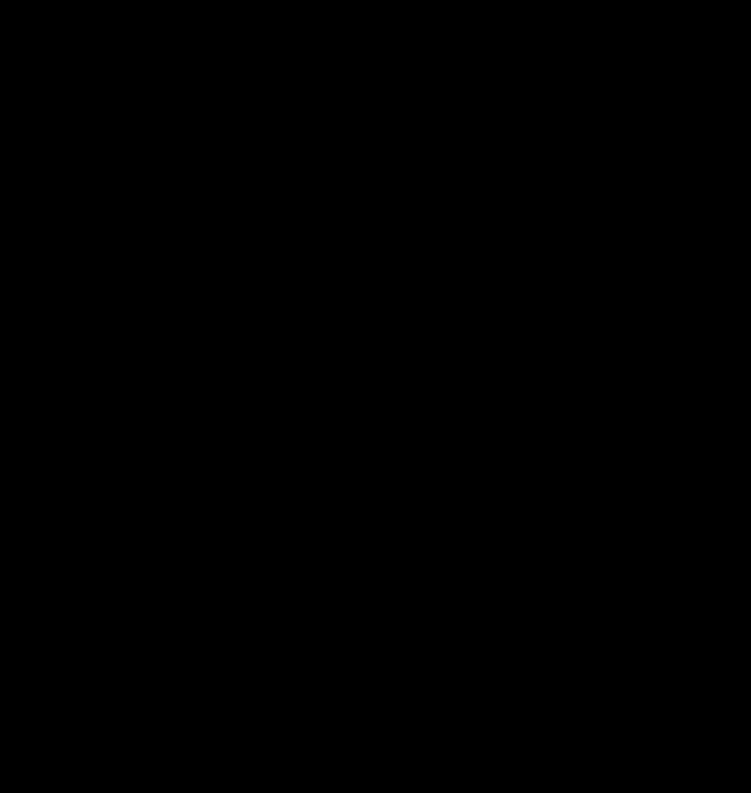
\includegraphics[scale=0.3]{drawing}
\caption{Complete undirected graph with 5 nodes}
\end{figure}\label{fig1}


\noindent


\medskip\noindent
The number of nodes in the graph is stored in a constant $n$:
\begin{verbatim}
const n = 5.
\end{verbatim}

\medskip\noindent
The number $K$ is also a constant:
\begin{verbatim}
const k = 2.
\end{verbatim} 

\medskip\noindent
The nodes of the graph are represented with a type $node$.

\begin{verbatim}
type node = {1..n}.
\end{verbatim}


\medskip\noindent
The edges of the graph are represented with the facts below. The atom $edge(i,j)$ for integers $i$ and $j$ is true if and only if there is an edge from node $i$ to node $j$ in the graph. The edges are defined as follows\DIFdelbegin \footnote{\DIFdel{for this example we could also define the edges using a single rule }\texttt{\DIFdel{edge(node X, node Y)}}%DIFAUXCMD
\DIFdel{, however we use a more sophisticated description for demonstration purpose. Similar rules can be used to define, for example, graphs with double ring topologies.}}  %DIFAUXCMD
\addtocounter{footnote}{-1}%DIFAUXCMD
\DIFdelend :

\DIFdelbegin %DIFDELCMD < \begin{verbatim}%DIFDELCMD < 
%DIFDELCMD < edge(node X, node Y) if X%n = (Y+1)%n.
%DIFDELCMD < edge(node X, node Y) if X%n = (Y+2)%n.
%DIFDELCMD < \end{verbatim}
%DIFDELCMD < %%%
\DIFdelend \DIFaddbegin \begin{verbatim}
edge(node X, node Y) if X%n = (Y+1)%n.
edge(node X, node Y) if X%n = (Y+2)%n.
edge(node X, node Y) if edges(X,Y) 
\end{verbatim}
\DIFaddend 

\DIFaddbegin \noindent
\DIFadd{where the last rule is needed to represent the undirectedness of the graph.
}\DIFaddend \medskip\noindent
We will check $K-connectedness$ by trying to remove up to $K-1$ nodes from the graph and checking whether the graphs remains connected.
For a node $N$ \texttt{removed(N)} is true if $N$ is removed from the graph. Any node may be removed from the graph:

\begin{verbatim}
maybe removed(node N).
\end{verbatim}   

\medskip\noindent
We are only interesting in the models where less than $K$ nodes are removed:

\begin{verbatim}
0 <= |{removed(node N)}| <= k-1.
\end{verbatim}

\medskip\noindent
To defined the connectedness of a graph, we first define a \texttt{reachable(X,Y)} relation, which is true if and only if there exists a path from $X$ to $Y$ in the graph not containing removed nodes:

\medskip\noindent
Any node which wasn't removed is reachable from itself:
\begin{verbatim}
reachable(node X, X) if not removed(X).
\end{verbatim}

\medskip\noindent
A node $Y$ is reachable from node $X$ if they are both not removed and there is an edge from $X$ to $Y$:
\begin{verbatim}
reachable(node X,node Y) if edge(X,Y) 
                            and not removed(X) 
                            and not removed(Y). 
\end{verbatim}

\medskip\noindent
\DIFdelbegin \DIFdel{A }\DIFdelend \DIFaddbegin 

\DIFadd{To define reachability for nodes not connected by an edge, we need an auxiliary relation $reachable\_through(X,Z,Y)$ which says
"a }\DIFaddend node $Y$ is reachable from node $X$ \DIFdelbegin \DIFdel{if there exists a }\DIFdelend \DIFaddbegin \DIFadd{through }\DIFaddend node $Z$\DIFaddbegin \DIFadd{".
}

\DIFadd{$reachable\_through(X,Z,Y)$ holds if $Z$ is }\DIFaddend reachable from $X$\DIFdelbegin \DIFdel{such that }\DIFdelend \DIFaddbegin \DIFadd{, }\DIFaddend $Y$ is reachable from $Z$ and none of the nodes $X$,$Y$,$Z$ was removed:

\DIFdelbegin %DIFDELCMD < \begin{verbatim}%DIFDELCMD < 
%DIFDELCMD < reachable(node X,node Y) if reachable(X,some node Z)
%DIFDELCMD <                             and reachable(Z,Y) 
%DIFDELCMD <                             and not removed(X) 
%DIFDELCMD <                             and not removed(Y) 
%DIFDELCMD <                             and not removed(Z).
%DIFDELCMD < \end{verbatim}
%DIFDELCMD < %%%
\DIFdelend \DIFaddbegin \begin{verbatim}
reachable_though(node X,node Z, node Y) if reachable(X,Z),              
                            and reachable(Z,Y) 
                            and not removed(X) 
                            and not removed(Y) 
                            and not removed(Z).
\end{verbatim}

\DIFadd{Finally, a node $Y$ is reachable from node $X$ if $Y$ is reachable from $X$ through some node:
}

\begin{verbatim}
reachable(node X, node Y)
                if reachable_through(node X, some node, node Y).
\end{verbatim} 
\DIFaddend 


\medskip\noindent
The graph is k-connected if any two nodes  that were not removed are reachable from each other.
We next define the disconnected relation: the graph is disconnected if there exists a pair of nodes which are not reachable from
each other.

\DIFdelbegin %DIFDELCMD < \begin{verbatim}%DIFDELCMD < 
%DIFDELCMD < disconnected if    not reachable(some node X, some node Y) 
%DIFDELCMD <                    and not removed(X)
%DIFDELCMD <                    and not removed(Y).                
%DIFDELCMD < \end{verbatim}
%DIFDELCMD < %%%
\DIFdelend \DIFaddbegin \begin{verbatim}
disconnected(node X, node Y) if not reachable(X, Y) 
                   and not removed(X)
                   and not removed(Y).                

disconnected_graph if disconnected(some node, some node).   
\end{verbatim}
\DIFaddend If there exists at least one way to remove at most $k-1$ such that the graph is disconnected, the graph is not k-connected.
We can check this by, first, putting a constraint requiring the graph to be disconnected:

\DIFdelbegin %DIFDELCMD < \begin{verbatim}%DIFDELCMD < 
%DIFDELCMD < 1<=|{disconnected}|<=1.
%DIFDELCMD < \end{verbatim}
%DIFDELCMD < %%%
\DIFdelend \DIFaddbegin \begin{verbatim}
1<=|{disconnected_graph}|<=1.
\end{verbatim}
\DIFaddend 

\medskip\noindent
The graph is not $K$-connected if and only there exists at least one model of the program.

\medskip\noindent
The program has no models for $k<=4$ but has a model for $k=5$. That is, the graph on figure \ref{fig1} is $4-connected$ but not $5-connected$ (for example, the nodes \{2,3,4,5\} can be removed from the graph to make it disconnected).


\DIFaddbegin \DIFadd{A complete program for this example is given in appendix \ref{B}
}

 

\DIFaddend \pagebreak
\appendix
\section{L program for checking safety obligations}\label{A}

\DIFdelbegin %DIFDELCMD < \begin{verbatim}%DIFDELCMD < 
%DIFDELCMD < 

%DIFDELCMD < type requiredInspection = {epa_i_652_6B_714_A, epa_i_652_6B_714_B}.
%DIFDELCMD < type epaSafetyHearing = {}.
%DIFDELCMD < type requiredFromEPA714 = {} .
%DIFDELCMD < type epaFine_j_652_6B_710_C = {}.
%DIFDELCMD < 

%DIFDELCMD < 
%DIFDELCMD < safetyObligationsMet if
%DIFDELCMD <    requirementsCertified and
%DIFDELCMD <    validationProcessFollowed and
%DIFDELCMD <    passed(every requiredInspection).
%DIFDELCMD < 

%DIFDELCMD < requirementsCertified if
%DIFDELCMD <    requirementsSound and
%DIFDELCMD <    requirementsComplete.
%DIFDELCMD < 

%DIFDELCMD < validationProcessFollowed if
%DIFDELCMD <    satisfied(code_825_A_6_A) and
%DIFDELCMD <    satisfied(code_825_A_6_B) and
%DIFDELCMD <    satisfied(code_825_A_6_C) and
%DIFDELCMD <    satisfied(code_825_A_6_D) and
%DIFDELCMD <    satisfied(code_825_A_6_E).
%DIFDELCMD < 

%DIFDELCMD < 
%DIFDELCMD < passed(epa_i_652_6B_714_A) if
%DIFDELCMD <    completed(every requiredFromEPA714) and
%DIFDELCMD <    not pending(every epaFine_j_652_6B_710_C).
%DIFDELCMD < 

%DIFDELCMD < 
%DIFDELCMD < passed(epa_i_652_6B_714_B) if
%DIFDELCMD <    paid(every epaFine_j_652_6B_710_C).
%DIFDELCMD < 

%DIFDELCMD < \end{verbatim}
%DIFDELCMD < %%%
\DIFdelend \DIFaddbegin \begin{verbatim}

type requiredInspection = {epa_i_652_6B_714_A, epa_i_652_6B_714_B}.
type epaSafetyHearing = {es1,es2}.
type requiredFromEPA714 = {rfe1} .
type epaFine_j_652_6B_710_C = {efj1,efj2,efj3}.


safetyObligationsMet if
   requirementsCertified and
   validationProcessFollowed and
   passed(every requiredInspection).

requirementsCertified if
   requirementsSound and
   requirementsComplete.

validationProcessFollowed if
   satisfied(code_825_A_6_A) and
   satisfied(code_825_A_6_B) and
   satisfied(code_825_A_6_C) and
   satisfied(code_825_A_6_D) and
   satisfied(code_825_A_6_E).


passed(epaFine_j_652_6B_710_C H) if not pending(H).

passed(epa_i_652_6B_714_A) if
   completed(every requiredFromEPA714) and
   passed(every epaFine_j_652_6B_710_C).


passed(epa_i_652_6B_714_B) if
   paid(every epaFine_j_652_6B_710_C).
\end{verbatim}
\DIFaddend \pagebreak
\section{L program for checking K-connectivity of a graph}\label{B}
\DIFdelbegin %DIFDELCMD < \begin{verbatim}%DIFDELCMD < 
%DIFDELCMD < const n = 5.
%DIFDELCMD < const k = 2.
%DIFDELCMD < 

%DIFDELCMD < type node = {1..n}.
%DIFDELCMD < 

%DIFDELCMD < edge(node X, node Y) if X%n = (Y+1)%n.
%DIFDELCMD < edge(node X, node Y) if X%n = (Y+2)%n.
%DIFDELCMD < 

%DIFDELCMD < maybe removed(node N).
%DIFDELCMD < 

%DIFDELCMD < 0 <= |{removed(node N)}| <= k-1.
%DIFDELCMD < 

%DIFDELCMD < reachable(node X, X) if not removed(X).
%DIFDELCMD < reachable(node X,node Y) if edge(X,Y) 
%DIFDELCMD <                             and not removed(X) 
%DIFDELCMD <                             and not removed(Y). 
%DIFDELCMD < reachable(node X,node Y) if reachable(X,some node Z)
%DIFDELCMD <                             and reachable(Z,Y) 
%DIFDELCMD <                             and not removed(X) 
%DIFDELCMD <                             and not removed(Y) 
%DIFDELCMD <                             and not removed(Z).
%DIFDELCMD < 

%DIFDELCMD < disconnected if    not reachable(some node X, some node Y) 
%DIFDELCMD <                    and not removed(X)
%DIFDELCMD <                    and not removed(Y).                
%DIFDELCMD < 

%DIFDELCMD < 1<=|{disconnected}|<=1.
%DIFDELCMD < \end{verbatim}
%DIFDELCMD < %%%
\DIFdelend \DIFaddbegin \begin{verbatim}
const n = 6.
const k = 5.

type node = {1..n}.
edge(node X, node Y) if X%n = (Y+1)%n.
edge(node X, node Y) if X%n = (Y+2)%n.
edge(node X, node Y) if edge(Y,X).

maybe removed(node N).
0 <= |{removed(node N)}| <= k-1.
reachable(node X, X) if not removed(X).

reachable(node X,node Y) if edge(X,Y) 
                            and not removed(X)                                                                                                               
                            and not removed(Y). 

reachable_through(node X,node Z, node Y) if reachable(X,Z)
                            and reachable(Z,Y) 
                            and not removed(X) 
                            and not removed(Y) 
                            and not removed(Z).


reachable(node X,node Y) if reachable_through(X,some node, Y).

disconnected(node X, node Y)  if    not reachable(X, Y) 
                   and not removed(X)
                   and not removed(Y).                


disconnected_graph  if   disconnected(some node, some node).                 


1<=|{disconnected_graph}|<=1.
\end{verbatim}
\DIFaddend %\bibliography{mylib}
%\bibliographystyle{plain}


\end{document}


%%% Local Variables:
%%% mode: latex
%%% TeX-master: t
%%% End:
